\documentclass{report}
\usepackage{amsmath}
\usepackage{amsfonts}
\usepackage{mathabx}
\usepackage{amsthm}
\usepackage{amssymb}
\usepackage{framed}
\usepackage{relsize}
\usepackage{subfig}
\usepackage{graphicx}
\graphicspath{ {images/}}
\usepackage{subcaption}
\usepackage{enumerate}
\usepackage{booktabs}

\usepackage[
style=authoryear,
citestyle=authoryear,
maxcitenames=1,
maxbibnames=6
]{biblatex}
\addbibresource{project.bib}
\bibliography{project}

\usepackage[usenames,dvipsnames]{color}
\usepackage{tikz}
\usepackage{listings}
\lstset{language=Python, breaklines=true}  
\usepackage{fancyhdr}
\setlength{\parindent}{0pt}
\pagestyle{fancy}
\fancyhf{}
\fancyhead[R]{Michael Redman, CID:\ 00826863}
\fancyfoot[C]{\thepage}
\begin{document}
\title{Detecting pathologies in spatiotemporal data}
\author{Michael Redman, CID:\ 0082686\textbf{3}}
\date{December 2016}

\maketitle

\tableofcontents

\chapter{Introduction}

The identification of unusual patterns of disease is of obvious importance in public health. Discrepencies in the relative risk of disease incidence between regions will both inform the allocation of medical resources and motivate investigations over possible environmental exposure. \\

 The detection of such discrepencies is often done by the use of disease mapping studies which aggregate the recorded incidents of the disease of interest over time, and compare the total counts between regions. Public health information systems now record this data indexed to such a fine degree of granularity that the detection of risk factors which act at a very local level, such as hazardous industrial waste, can be feasably indentified. However this fine-grained approach will leave the examined regions with very low incidence, which can hinder the isolation of the signal from the noise, hence the use of time aggregated values. However, in doing this we relinquish any potential information that a temporal trend may afford us. In fact, as described in \cite{stability}, the nature of the temporal trend may suggest anomalities related to very different kinds risk factors. A region which conforms to a similar temporal trend as the others---for example a seasonal factor---but at a higher rate would imply a disparity which acts over the whole time period, such as an enviromental issue or a sociodemographic difference. While a region which acts wildly without regard to the general trend might suggest a more acute issue is at play, like an outbreak. \\

Consequently, in this project we will be looking at data that is indexed in both space and time. Additionally in any model that we implement, we wish to be able to control for any known covariates which may influence the risk within a given region. For example some regions will be more populous, while others may contain proportionally more at-risk peoples, so it would be wise to have some method of setting the expected counts by region. \\

A variety of methods have been investigated in these contexts. One of the most simple is that of scan statistics. This procedure, implemented in software such as SaTScan, seeks to identify clusters which can not be explained by the base process -- in our case typically an inhomogenous Poisson process. It does this by evaluating all possible ``windows'' in turn, where a given window will include the region in question and its ``neighbours'' both spatially and temporally. This forms a kind of cylinder which acts to smooth the observed counts in space and time, allowing the sparse data as described earlier to be examined without the noise overwhelming any underlying spatial heterogenicity. This method is descibed in detail and applied to epidemiological data in \cite{scan}. While offering an improvement over pointwise evaluation, spatial scan statistics by nature of this smoothing construction are limited in their ability to detect abnormalities at the individual level, i.e. isolated to a particular region (\cite{baystdetect}).  \\

Control chart based methods offer both relatively fast computation times and the ability to specifically identify abnormal temporal trends. These, in the simplest of terms, are graphs we construct combined with a decision rule to classify whether a process is in `in-control' or `out-of-control'. Versions such as CUSUM are often designed for step detection -- the identification of abrupt jumps in rate of the process. When looking at longer time periods, this is exactly the type of pathology one might expect. The regions which now show atypical trends should still have exhibited normal behaviour most of the time, the problem is to decide when such heterogeneity in the process is substantive.  Another advantage is, as the techinique is sequential in nature, the sample size of the items in consideration need not be fixed in advance.  \\

The most natural way to frame our problem is by the construction of a hierachical model. In this method we perform inference on a latent variable---within a complex model---which indicates the ``unusalness'' of a point or group of points. This Bayesian approach compells us to express our assumptions about the data generatively, which confers a number of advantages. Firstly, it is often the case in discriminative models that the choice of method is implicitly performing shrinkage, without this being made explicit or even realized by the modeler. For an intereting example see \cite{stoch}. Thinking generatively forces us to be clear about our assumptions. Secondly, real world epidemiological data will presumably not supply the true response variable, that is, whether or not a region is genuinely anomalous. This abscence of training means we need our model to provide reasonable estimates immediately, rather than at some asymptotic limit. This advantage can be seen in, for example, \cite{ng}. Thirdly, the parameters of a Bayesian model are far more readily interpretable that those in a non-generative setting, which could allow for further inference beyond the identification of abnormal regions, e.g. the nature and extent of the deviation from what was expected. And lastly,
 the Bayesian framework naturally allows the addition of futher assumptions and complexity. For example, \cite{banerjee} extends spatiotemporal models to the modelling of multiple diseases via the introduction of a shared `frailty' term. \\

The examination, implementation and comparison of these Bayesian methods with discriminative models, specifically control charts, is the focus of this project. \\

Working on simulated data, we first implement a CUSUM based classifier and suggest a novel(?) specification of the `in-control' process. With the efficiency of the method being of great importance, we implement the computations from scratch in Fortran rather than modifying the existing statistical routines in R. \\

Then, turning to Bayesian methods, we examine the general structure of the models employed in the literature and how this standard is well suited to the particular challenges of our problem. In particular, the favored priors for the smoothing of the data are reviewed. The difficulties and subtleties of computaion are addressed in detail, as are some of the superior techniques that have been developed in the past few years. \\

We examine BaySTDetect, one of the existing models in the literature, discussing the rationales behind the construction of the model and the `cutting of feedback' that's employed -- where we demonstrate that this particular choice is fundamental to it's success. Rather than use the standard MCMC software in the field, we implement the model in Stan using Hamiltonial Monte Carlo and combine the submodels directly through the likelihoods. We show that this can lead to order of magnitude speed-ups over the original implementation in \cite{baystdetect}. \\

We then suggest a new model, based on \cite{stability}, that works fully within the Bayesian framework by identifying an excess in the variance which can not be explained by the shared random effects. Implementing this model, again in Stan, we show that this model obtains good results, despite not being the way in which our simulated data were originally created. However, as suggested in \cite{best2005comparison}, models of this kind may oversmooth the counts spatially. We demonstrate this by simulating a new set of data where the regions to be `unusual' are selected sequentially via a preferential attachment scheme and showing that our model performs poorly in this context. \\

Finally we compare the use three models on both sets of data with respect to their speed, false postive rate and power.

\chapter{Simulated data}

In order to test the accuracy of any potential models we need some data that exhibits the type of pathological trends that we wish to identify. The following data was graciously supplied by Areti Boulieri.

\section{Specification}

A real dataset of asthma hospitalisation counts was used to contruct the expected rates, adjusted by regional demographics by age and sex, for the 221 Clinical Commisioning Groups in England. These are the expected counts that we will standardize against when attempting to identify abnormalities. We denote these values throughout by $E_{i}, \text{ for } i=1,\ldots,221$. A plot that we generated to show the distribution of these values across the regions can be seen in fig \ref{}  \\

A binomial random variable might be the most principled choice of response but the expected counts we have calculated are large enough for using a Poisson response to be essentially equivalent. Indeed this is the most popular choice in the literature. The data was generated across 15 time points, so our values are drawn from
\begin{equation}
Y_{i,t} \; \sim \; \operatorname{Poisson}(E_i \cdot \mu_{i,t}), \ \ \ \ i=1,\ldots,221 \ \ \ \ t=1,\ldots,15
\end{equation} 

where $\mu_{i,t}$ allows us to add random effects to our model. \\

These random effects are used to add additional natural variation to the counts, where the direction of this variation is in some sense shared between `similar' regions or time points. We seperate these effects into those that describe the temporal trend and those which affect the spatial heterogeneity. So for the temporal trend we of course expect adjacent time points to be similar. This is achieved in this data by sampling from a one-dimensional Gaussian random walk
\begin{equation}
\xi_{1:15} \; \sim \; \operatorname{RW1}(\sigma_{\xi}^2).
\end{equation}

Additionally, we would expect regions which are close to each other to be similar. The data generation incorporated this assumption by the use of the BYM prior, first defined in \cite{bym},
\begin{equation}
\lambda_{1:211} \; \sim \; \operatorname{BYM}(W, \sigma_{\lambda}^2, \sigma_v^2) 
\end{equation}
which is a multivariate normal distribution
\begin{equation}
\lambda_{1:211} \; \sim \; \cal{N}(v_{1:211}, I_{211}\sigma_{\lambda}^2)
\end{equation} 
where the mean vector is drawn from an \emph{intrinsically autoregressive} process
\begin{equation}
v_{1:211} \; \sim \; \operatorname{IAR}(W, \sigma_v^2)
\end{equation}
which is a Markov random field where areas that are adjacent (according to an adjacency matrix $W$) are more similar to those further away. The precise specification of the BYM prior is discussed in section \ref{carmodel}. \\

The presumed sources of these random effects will determine how we wish for them to influence the generation of the data. In this dataset it is assumed that the temporal and spatial effects will work multiplicatively, where increases in one will magnify the effect of the other. Therefore, given our samples from the aformentioned distributions, we calculate $\mu_{i,t}$ additively on the $\log$ scale
\begin{equation}
\log{(\mu_{i,t})} = \lambda_i + \xi_t \ \ \ \ i=1,\ldots,221 \ \ \ \ t=1,\ldots,15
\end{equation}

In total, this scheme describes a method of generating random variables that has the features one would expect of spatiotemporal disease incidence. We now need to modify a selection of the regions to resemble a regions we would expect to be unusual. \\

Fifteen of the regions were chosen according to the 10th, 25th, 50th, 75th and 90th percentiles of the median expected counts over time, with three regions per percentile. At each percentile the three regions were selected corresponding to one of three levels of spatial risk, i.e. the generated spatial effect $\lambda_{1:211}$, low (10th-30th percentiles), medium (45th-55th percentile) and high (70th-90th percentiles). This was done to ensure that the unusual regions were spread evenly given the underlying levels of risk. \\

To make these regions unusual they were given a deviant temporal trend. This was done by modifying the temporal trends of these regions manually, where---writing the original trend as $g(t)$ and the modified trend as $g^*(t)$---we have:
\begin{align}
g^*(t) &= g(t) + \log(2) && t = 1, 10, 11 \\ 
g^*(t) &= g(t) - \log(2) && t = 5, 15
\end{align}

This has the effect of either doubling or halving the expected counts depending on the time point. The resulting temporal trend compared to the original can be seen in figure \ref{fig:timeeffects}. \\

 N.B. All of the unusual regions exhibit the same deviation, which is probably an unrealistic assumption. However, by the way that they're defined, it is clear that the models used in this project should not perform better because of this fact. 

\begin{figure}
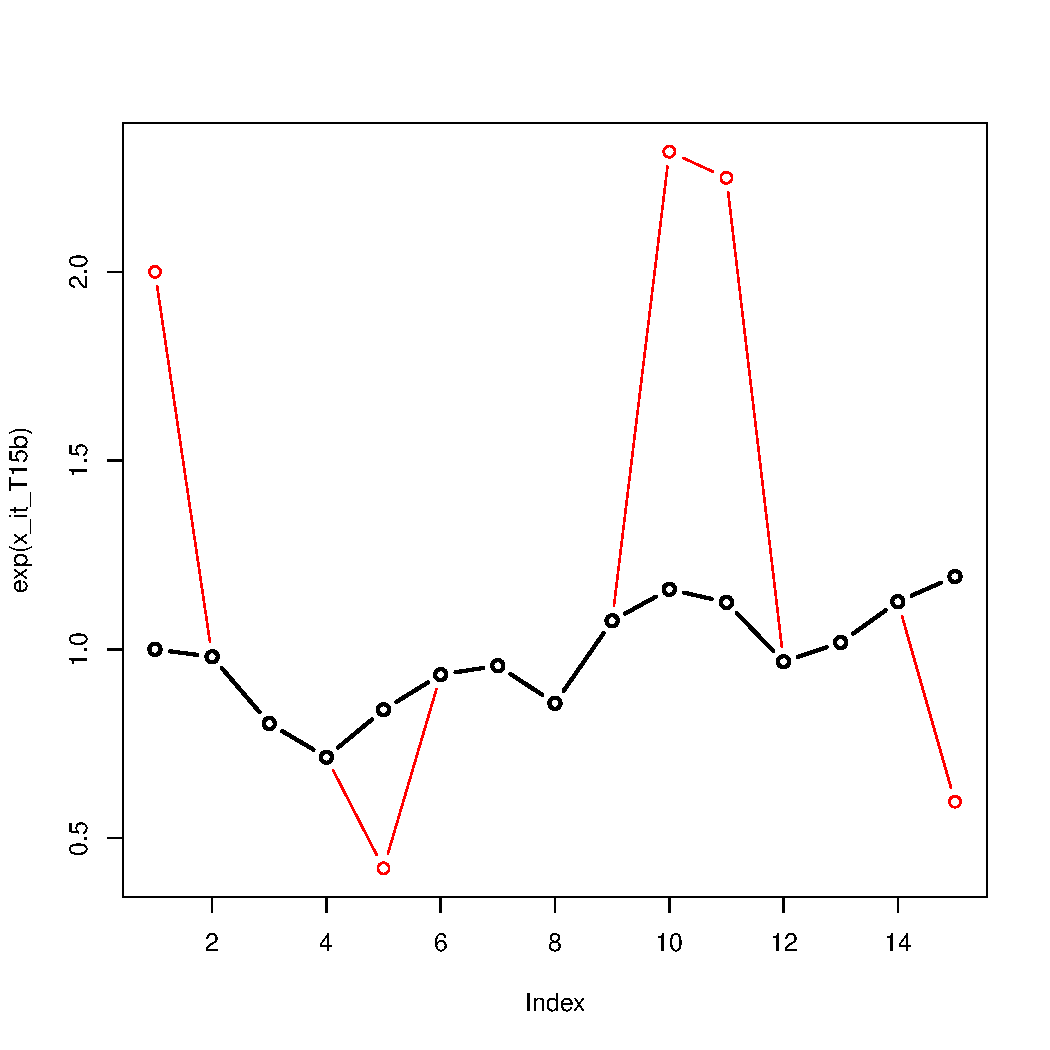
\includegraphics[scale=0.5]{plot_time_effects}
\label{fig:timeeffects}
\centering
\end{figure}

\begin{itemize}
\item Check this trend with Marta as the word document and pictured trend are different.
\end{itemize}

\section{Cleaning and wrangling}

Of the 211 regions only one one had no neighbours, the Isle of Wight. As this will complicate some of the smoothing calculations we need to perform for the Bayesian procedures (and the Isle of Wight was not one of those selected as unusual), the region was removed to simplify calculations.

Shape data for the 211 Clinical Commisioning Groups plus wales was provided by CITE HERE. The regions of Wales and the Isle of Wight were of course removed. The shapefiles were imported and edited using the package \emph{rgdal} created by \cite{shaperead}. Then, using the package \emph{spdep} created by \cite{shape}, the shapefile was used to generate an object which calculates all of the adjacent regions for each region. Then this object was converted into into an adjacency matrix $W$ such that
\begin{equation*}
{(W)}_{ij} &= 
\begin{cases}
1, \ \ i \leftrightarrow j \\
0, \ \ \textrm{otherwise}
\end{cases}
\end{equation*}
where the double arrow signifies adjacency. The result of this procedure can be seen over the original shapedata in fig \ref{adj}.


 
 An adjacency matrix calculated from the shape data. We had no data for wales so it was removed from the shapedata.

\begin{figure}
\centering
\subfloat[Adjacency]{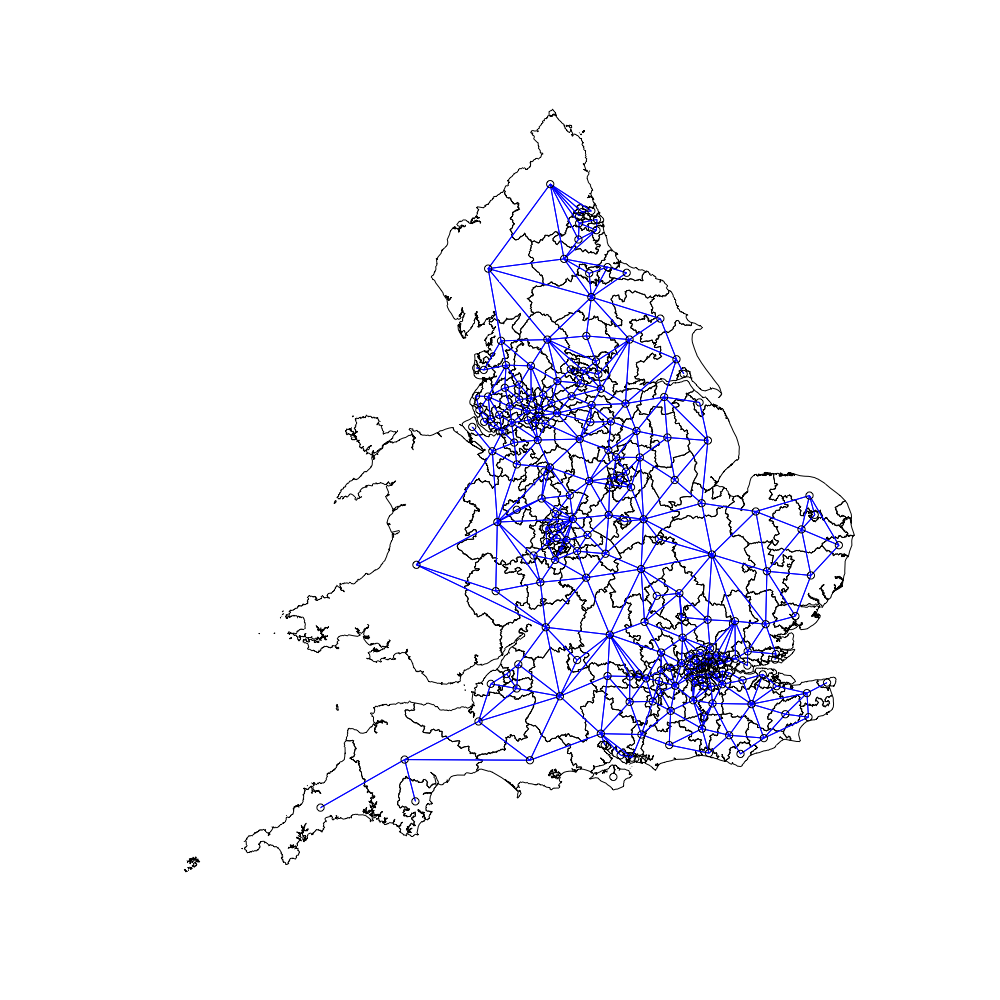
\includegraphics[width=0.5\textwidth]{adjacency}}
\subfloat[Expected]{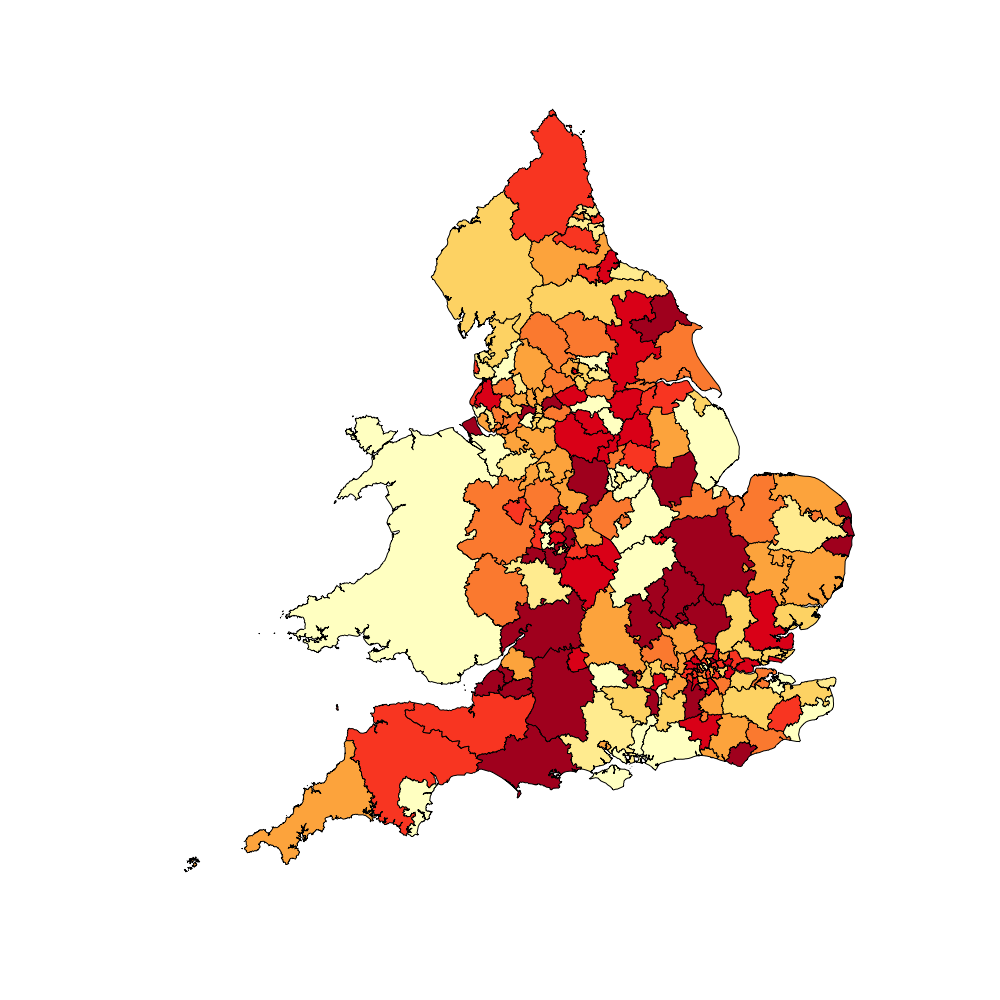
\includegraphics[width=0.5\textwidth]{expected}}
\caption{Mapped data}
\end{figure}

\chapter{CUSUM}

The use of control charts are widespead in the area of statistical quality control and have recently increasingly found use in fields such as epidemiology, e.g. . Their relative simplicity and ease of computation compared to most other methods makes them an ideal model to compare against, in order to observe any gains we might obtain from more complex modelling.

\begin{itemize}
\item Mention that the process is sequential and so can be calculated as we go.
\item Spatial CUSUM
\end{itemize}

We will specifically be looking at the use of CUSUM models, which seek to identify a qualitative change in the nature of a time series via the evaluation of the cumulative of a relavant test statistic. We define $S_t$ as the value of the control chart at time $t$ and progress its value as follows
\begin{gather}
S_0 = 0 \\
S_{t+1} = \max{(0, S_t + K_t)}.
\end{gather}

Where $K_t$ is the value of some statistic calculated at time point $t$. We will use the $\log$ of the ratio between the likelihoods of the data, at the time point, under an ``in-control'' and an ``out-of-control'' Poisson process. So if likelihood of the ``out-of-control'' rate is greater than the ``in-control'' then the value of $S_t$ will increase and vice-versa. The logarithms are taken to minimise floating-point arithmetic issues as the densities will often be very small. We then signal that the process is pathological if the value of $S_t$ exceeds some threshold value $h$. \\

This leaves us to come up with sensible methods of generating the ``in-control'' and ``out-of-control'' rates and the threshold value that we trigger at. With the data that we area examining in this project we have the expected values of the disease rates in each region and could use these for the values of the ``in-control'' rate but this would neglat the fact that we expect the incident counts at each region to vary over time and---importantly---this is not neccasarily pathological behaviour. It is instead a temporal trend which differs from some general (here country-wide) trend which we wish to detect. Therefore the method we propose here is to construct a general temporal trend from an average across the regions and to weight this trend per region by that regions expected counts. \\

So for the data $Y_{i,t}, \ i = 1, \ldots, R, \ t = 1, \ldots, T$ we normalize the temporal pattern of each regions by its expect count $E_{i}$ as follows
\begin{equation}
\tilde{Y}_{i, t} = \frac{Y_{i, t}}{E_{i}}, \ \ \ \ i = 1, \ldots, R, \ t = 1, \ldots, T.
\end{equation} 

We then construct the ``in-control'' rate for each region $I_{i, t}$ as described
\begin{equation}
I_{i, t} = E_i \cdot \frac{1}{R} \sum_{i=1}^N \tilde{Y}_{i, t}, \ \ \ \ i = 1, \ldots, R, \ t = 1, \ldots, T.
\end{equation}

For simplicity we only consider the case of abnormally high count rates and ignore artificially low counts but this could be incorporated into the CUSUM model if desired. So to define the ``out-of-control'' rate it makes sense to follow the same temporal trend but with a modified general rate. We do this by calculating the ``out-of-control'' rate $O_{i,t}$ as a multiple of the ``in-control'' as follows
\begin{equation}
O_{i,t} = \lambda \cdot I_{i,t}, \ \ \ \  i = 1, \ldots, R, \ t = 1, \ldots, T.
\end{equation} 
with $\lambda > 1$. \\

Now for a given value of $\lambda$ we need a threshold level at which to signal. This can be done by caluclating the average-run length (ARL) which is the expected length of the series between flags of the model. The ARL on the ``in-control'' rate will then give a measure of the false positives for a given threshold $h$, which we can optimize with respect to. As the length of the series we are examining is fixed and the calculation of an ARL would not be clearly defined for a series of varying expectation we will not use the ARL metric here. Instead we simply simulate the ``in-control'' sequence for each region $n$ times and find the smallest value of $h$ for which the the false-postive rate is below 1\%. \\

The setup as described was implemented as a Python class acting as a wrapper to a series of subroutines in Fortran via F2PY\footnote{I originally wrote the entire process in Python but the calculation of the $h$ values was far too slow to be practical. The original code can be on my Github.}. The code can be found in the appendix. \\

This CUSUM process was applied to the asthma data with the ratio $\lambda$ set to $1.5$, indicating we consider the ``out-of-control'' rate to be 50\% greater than the ``in-control'', with each regions temporal pattern being simulated 10,000 times to determine the optimal threshold values. This identified 25 regions as ``out-of-control'' out of the total 210, giving a false-negative rate of 0\% and false-positive rate of 5.2\%. \\

To conclude, while CUSUM correctly identified the unusual regions, we have a high false-positive rate as the ``in-control'' likelihood was a poor approximation to the true likelihood for a number of regions.  

\section{The Bayesian Framework}

A sensible way of improving on this would be to use a generative model which incorporates both a flexibility that describes our uncertainty around the parameterization of the model and makes explicit our beliefs as to the structure of the data. This is most naturally done in the Bayesian framework, where we specify the model in terms of a likelihood which describes how we simulate the data based on a set of parameters and a collection of---possibly hierarchical---priors which describe our uncertainty about these parameters ex ante. 

\begin{enumerate}
\item Advantages of generative models
\item Advantages over frequentist approaches, e.g. mean/mode often terrible approximations, in part due to concentration of measure
\item Level of shrinkage attributable to closeness of prior structure to some ``true prior''
\item Bayes formula
\item Difficulty in evaluating integrals/expectations
\item Samples will converge to expectation (use betancourts conceptual into here)
\item Proposal density and preserving the pdf
\item Metropolis-hastings
\item Theory and issues including: large/small step sizes, large autocorrelation, slow exploration of the sample space, divergences
\item Gibbs sampleing and blocked gibbs: overcomes some element of dimensionality but poor for highly correlated variables, compounded by issues with 
\item Asymptotics not followed in finite time often
\item Quick talk about existing software
\item Hamiltonian monte carlo provides some solutions to many of these problems
\item In last few years (get exact) emergence of better algorithms, tuning and software have made using HMC practical. Not used in epidemiology much yet though. Different fields different amounts due to issues with discrete paramters etc. that we will address later.
\item Convergence statistics
\end{enumerate}

\begin{itemize}

\item Space-time seperability

\item Identification issuses in mixture model

\item Bayesian model selection

\item Prior on mixture component probability

\item Bayesian classification

\end{itemize}

\subsection{Hyperparameter priors}

\begin{itemize}

\item Gelman 2006 for variance parameters

\item Stan wiki for others

\end{itemize}

\subsection{Convergence statistics}

\begin{itemize}

\item Trace plot

\item Gelman-Rubin statistic

\item Multiple-chains are run not for computational benefits but to assess convergence

\item Gelman-Rubin-brooks plot

\item Lack of divergences---which are ``incredibly sensitive to the kind of pathologies that can obstruct geometric ergodicity'' 


\end{itemize}


\subsection{Hamiltonian Monte-Carlo}

The previous methods, while possessing the desired asymptotic properties, can---and do---take a long time to converge to the target distribution (infinity is a long time!). The aim of \emph{Hamiltonian Monte-Carlo} is to reduce the correlations between successive samples and so dramatically increase the effective sample size with minimal computational overhead. It does this by introducing an auxilliary variable and exploiting the interplay between this and the variables of the posterioir distribution within the framework of Hamiltonian mechanics.

\subsubsection{Background}

We write $q$ for the variables of the posterior distribution and introduce a new variable $p$ which we will call the \emph{momentum} of the system. Drawing from statistical mechanics, we know that for a given energy function of a system $E(\theta)$ we have the canonical ensemble
\begin{equation}
  p(\theta) = \frac{1}{Z} e^{-E(\theta)}.
\end{equation}

So defining a Hamiltonian of our system where the ``kiniteic energy'' is dependent on our momentum and the potential energy is dependent only on the posterioir:
\begin{equation}
  H(p, q) = \underbrace{T(p|q)}_{\text{Kinetic energy}} + \underbrace{V(q)}_{\text{Potential energy}}
\end{equation} 

looking at the canonical ensemble of the join distribution
\begin{align}
  \pi(p, q) &\;{\propto} \; e^{-H(p, q)} \\
          &= e^{-[T(p|q) + V(q)]} \\
          &= e^{-T(p|q)} \cdot e^{-V(q)} \\
          &\;{\propto} \; \pi(p|q) \cdot \pi(q) 
\end{align}

we see that the posterior and distribution of the momentum are seperable and so independent. This means that if we can sample from $\pi(p, q)$ then our choice of distirbution for the momentum will not effect the calculation of any expectations based on the samples of $q$. \\

Note that here we need a definition of potential energy which will give us back the posterior. Clearly the following satisfies this requirement
\begin{equation}
  V(q) = - \log \pi(q)
\end{equation}

So draws from $\pi(p, q)$ will allow us to make inferences on the $q$, but what advantages does the introduction of this auxilliary variable confer? Well, continuing with our intuition regarding a physical Hamiltonian system, we know that $p$ and $q$ are related by Hamilton's equations
\begin{align}
\frac{dq}{dt} &= \frac{\partial H}{\partial p} = \frac{\partial T}{\partial p} \\
\frac{dp}{dt} &= - \frac{\partial H}{\partial q} = - \frac{\partial T}{\partial q} - \frac{\partial V}{\partial q}
\end{align}

\begin{itemize}
  \item Finish off this bit more gracefully
\end{itemize}

\subsubsection{The Method}
Hamiltonian monte-carlo works, not by applying a transition over $q_i$, but by giving our starting point ``a kick'' in the form of a random momentum and sampling along the level set of constant energy (defined by the Hamiltonian) using Hamilton's equations to evolve the joint system. Then---after some number of steps---we stop, sample a new momentum, and explore the new phase space that this defines. \\

The questions now are obvious:

\begin{itemize}
\item \emph{How} do we evolve the joint system in accordance with Hamilton's equations? (Leapfrog)
\item Do we need to work out all of the partial deriavtives $\partial V/\partial q_i$ by hand? 
\item For how long should we explore each level set before sampling a new momentum?
\item What proposal density should we use for the momentum?
\item Why does this method lead to samples with less autocorrelation?
\end{itemize}

Other things to talk about:
\begin{itemize}
\item \emph{How} do we evolve the joint system in accordance with Hamilton's equations?
\item Do we need to work out all of the partial deriavtives $\partial V/\partial q_i$ by hand? 
\item For how long should we explore each level set before sampling a new momentum?
\item What proposal density should we use for the momentum?
\item Why does this method lead to samples with less autocorrelation?
\item Parameter tuning vs burn-in period
\end{itemize}

Other things to talk about:
\begin{itemize}

\item Rotational invariance

\item Include some diagrams from Michael Betancourt's papers

\end{itemize}

\subsection{General Model Form}

\begin{itemize}
\item Use best et al to summarise basic model form
\end{itemize}

\section{Smoothing}

Ideally we wish to identify potential local risk factors in the aetiology of a disease, say, carcenogenic hazard from industrial polution. So it's clear that the ability to incorporate a high level of spatial granularity in our model is of value in these contexts. However this comes with the trade-off of greater variance in the counts, making identification of abnormal temporal trends difficult, especially for diseases with low incidence. Therefore we need to employ an element of smoothing over the local neighbourhoods of each region. This can be done in a variety of methods. One possibility is the use of splines such as in (source here) but in this project we will primarily look at using a conditionally autoregressive prior.

\subsection{CAR models} \label{carmodel}

Markov random field.

Conditionally autoregressive models can be best understood when specified in terms in terms of their conditional distribution. 

\begin{equation}
v_i \ | \ v_j \ j \neq i \sim N(\alpha \cdot \bar{\mu_i}, \ \sigma_v^2/k_i)
\end{equation}

where $k_i$ is the number of neighbours adjacent to region $i$,

\begin{equation}
\bar{\mu}_i = \sum_{j \in \partial i} \frac{\mu_j}{k_i}
\end{equation}

and $\alpha$ is a parameter measuring the degree of spatial dependence. 

However as this specification is a markov random field and not a directed acyclic graph we can't use this definition in non-gibbs sampling methods \- we need the $v_i$ to be jointly specified. Thankfully it is possible for it to be expressed in terms of a multivariate normal distribution as follows,

\begin{equation}
v \ \sim \ N(0, \ \sigma_v^2 \cdot {[D(I_n - \alpha B)]}^{-1})
\end{equation}

where

\begin{align}
D &= \operatorname{diag}(k_i) \\
B &= D^{-1} W \\
{(W)}_{ij} &= 
\begin{cases}
1, \ \ i \leftrightarrow j \\
0, \ \ \textrm{otherwise}
\end{cases}
\end{align} 

It is intuitively clear that the precision matrix here is sparse and so naive calculations will be very inefficient -- see the section on computational considerations for some more sophisticated methods that we will use to simulate the distribution.

Cite \cite{car}

\begin{itemize}

\item Cite http://www.biostat.umn.edu/~brad/software/jbc.proofs.pdf

\item Write in terms of join distribution for non-gibs samplers.

\item Spatial dependence parameter $\alpha$ --- to prior or not to prior?

\item Intrinsically autoregressive model --- improper as covariance matrix is semi-definite

\end{itemize}

\subsection{BYM prior}

\begin{itemize}
\item CIte Besag York Mollie paper
\item Increases degrees of freedom for spatial componenet
\end{itemize}

\subsection{Temporal smoothing}

Similarly to in the spatial setting we can use a prior on the temporal component that assumes a level of similarity between adjacent regions -- here consecutive time points. The prior prefered here is the one dimensional random walk prior, which we will denote by
\begin{equation}
\xi_{1:T} \sim \operatorname{RW}(1)
\end{equation}

where the dimensionality will often be infered from the context. Note that this can be represented by a CAR model and is sometimes represented as such in the literature. 

\section{Individual trend model}

The first Bayesian model we wil consider is similar to that which is formed in Someone et al. In this setting we construct two alternate hypothesis for each region, one where the counts at the region are broadly in keeping with some ``global'' temporal trend (subject to localised spatial deviations captured with a conditionally autoregressive prior), and in the other the region has its own individual temporal trend. Then by some method of classification we sort the regions into those deemed most likely to follow the global model and those exhibiting behaviour more typical of the second model - and label these regions ``unusual''.

\subsection{Baystdetect and the cut function}

In the original paper \cite{baystdetect} the use of the cut function in the \emph{BUGS} language is employed to fit the two models to the data seperately and then the model selection is undertaken afterward. This method, which prevents the flow of information between the two models is defended in (Nicky Best presentation here) but has been met with some level of skepticism in the community, for example in Andrew Gelmans posts to the Stan mailing list here (insert link), as the analysis is not ``truly Bayesian''. Nethertheless, we examine this paradigm and compare it to fully Bayesian methods. 

\begin{itemize}
\item Include discussion of model averaging vs larger model
\item Cite Gelman et al 2013
\end{itemize}

\subsubsection{Model specification}

We denote the counts at region $i$ at time $t$ by $Y_{i,t}$ and model them by a Poisson process

\begin{equation}
Y_{i,t} \sim \operatorname{Poisson}(E_{i,t} \cdot \mu_{i,t})
\end{equation}

where $E_{it}$ is the expected count based on population numbers, demographics etc and $\mu_{i,t}$ is the rate parameter by which we impute the two models behaviours. This rate variable we parameterize additively on the log scale for both models as follows

\begin{equation}
\log{(\mu_{i,t})} = \begin{cases}
\ \lambda_{i} + \gamma_{t} \  (+ \  \alpha_0) & \textrm{Model 1 for all } i, t \\
\ u_{i} + \xi_{i,t} & \textrm{Model 2 for all } i, t
\end{cases}
\end{equation} 

Here we see that for Model 1 we assume space-time seperability in the rate paramater with the components given the following priors

\begin{align}
\alpha_0 &\sim \operatorname{Flat}(\mathbb{R}) \\
v_{1:N} &\sim \operatorname{CAR}(W, \sigma_v) \\
\lambda_{1:N} &\sim \operatorname{Normal}(v, \sigma_\lambda) \\
\gamma_{1:T} &\sim \operatorname{RW}(1)
\end{align}

We see here the BYM prior on the spatial component, imposing a smoothing constraint, and a one-dimensional random walk prior on the temporal component. 

The variance hyperparameters are given (insert prior here) as recomended in (possibly Gelman 2006). \\

For the second model we drop the assumption of space-time seperability and each region gets its own temporal trend as follows

\begin{equation}
i \in 1,\ldots,N \
\begin{cases}
\ u_i \sim \operatorname{Normal}(0, 1000) \\
\ \xi_{i, 1:T} \sim \operatorname{RW}(1) 
\end{cases}
\end{equation}

\subsection{Combining the models}

\begin{itemize}
\item BUGS can be used with a mixture component
\item In this case the likelihood can be worked out by hand with the probability of the mixture component prior
\item Describe likelihood code
\end{itemize}

\subsubsection{Implementation}

The two models were fit to the data using Hamiltonian Monte-Carlo in the \emph{Stan} package -- both for over 2000 samples over 4 chains after a ``warm-up'' period of 1000 samples. Gelman-Rubin statistics for all parameters were under 1.05 (find exact figure) indicating that the had chains converged. Additionally a visual inspection of the trace plots for some select parameters did not indicate any worrying pathalogical behaviour.

These two fits took under 5 minutes each to run after a short compilation which is a huge speed increase over typical \emph{BUGS} implementation.

\subsubsection{Classification and accuracy}

First looking at the general trend model we see that it has accurately identified the global temporal trend. 

\begin{figure}
\centering
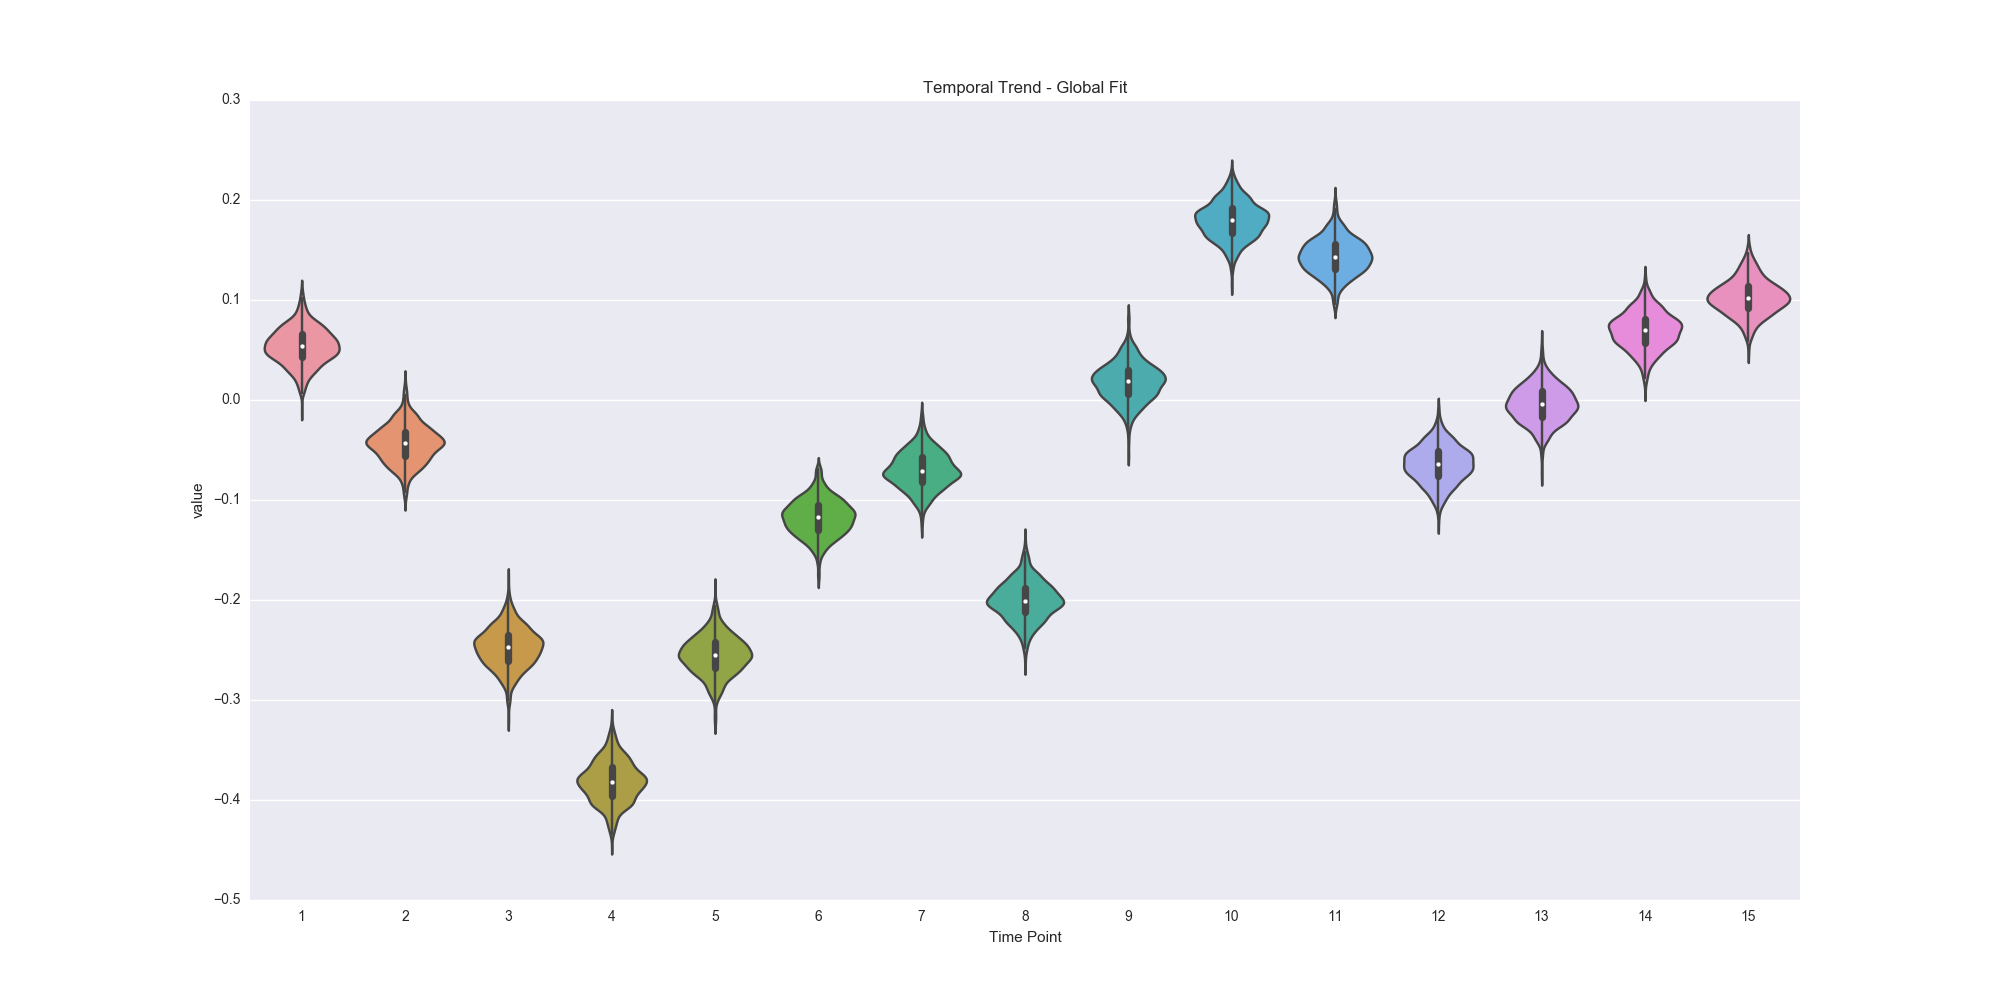
\includegraphics[width=\textwidth]{global_temporal}
\end{figure}

\subsection{Fully Bayesian model}

\begin{itemize}
\item Can be fit fully in Stan
\item Reference the use of Rao-Blackwellization
\item Graph the temporal components failure
\end{itemize}

\section{Excess variability model}

The second Bayesian model we will look at also attempts to classify the regions, into typical and atypical sets, using a mixture model. Here our abnormal regions, rather than coming from an individual temporal trend, simply have excess inseperable spatio-temporal variance. Some potential advantages of such a model compared to Baystdetect are immediately clear:
\begin{itemize}
\item It's relative simplicity allows for easier computation
\item It is not immediately clear that an abnormal temporal trend is symptomatic of an endemic problem --- variance is a more straightforwardly interpretable parameter
\item Identification issues
\item Mixture model issues reduced due to setup of variance
\end{itemize}

\subsection{Model specification}

The model is similar to that of \cite{stability}, but with a mixture component that's hierachical at the regional level. Like before we model the counts as a Poisson process, $Y_{i,t} \sim \operatorname{Poisson}(E_{i,t} \cdot \mu_{i,t})$, with a rate parameter defined additively on the log-scale

\begin{equation}
\log(\mu_{i,t}) = \lambda_i + \gamma_t + \psi_{i,t}
\end{equation}

where, as before,
\begin{align}
v_{1:N} &\sim \operatorname{CAR}(W, \sigma_v^2) \\
\lambda_{1:N} &\sim \operatorname{Normal}(v, \sigma_\lambda^2) \\
\gamma_{1:T} &\sim \operatorname{RW}(1).
\end{align}

We see the new component $\psi$ captures a level of space-time inseperability to the counts. At every point $(i, t)$ each component is modeled as coming from a mixture of two normal distributions, with the mixture component at the regional level,
\begin{equation}
\psi_{i,t} \sim z_i \cdot \operatorname{Normal}(0, \tau_1^2) + (1 - z_i) \cdot \operatorname{Normal}(0, \tau_2^2)
\end{equation} 

where
\begin{equation}
  z_i \sim \operatorname{Bernoulli}(q_i)
\end{equation}

and the $q_i$ are given Uniform priors on (0, 1). Here we are marginilizing out the $z_i$ and instead performing inference on the $q_i$ which confers the advantages set out under the computational considerations section. The variance parameters are given half-normal priors, one a vague prior (representing the abnormal regions) and the other an informative prior which restricts the inseperable variance of the `normal' regions to be very limited. Identification issues and the label switching problem are avoided by defining the larger of the variances addivitely in terms of the smaller:
\begin{align}
  \tau_1 &\sim \operatorname{Normal}(0, 0.01) \cdot I(0, \infty) \\
  k &\sim \operatorname{Normal}(0, 100) \cdot I(0, \infty)
\end{align}
\begin{equation}
 \tau_2 = \tau_2 + k
\end{equation}

Here $I$ is the indicator function.

\subsection{Classification and accuracy}

This model was fit using HMC in \emph{Stan} 

\subsection{Over-smoothing}

\begin{itemize}
\item Expected disease trends will cluster
\item Model relies on finding unseperable variance but local high variance could be explained by CAR component
\item Need a model which smooths regions but is able to still identify clustered unusual areas
\end{itemize}

\subsection{Simulated Data}

\begin{itemize}
\item Preferential attachment scheme
\item Describe full data generation parameters and process
\item Include plots of temporal and spatial components
\end{itemize}

\section{Computational considerations}

\subsection{Basic Sampling methods}

\begin{itemize}

\item Mainly using stan for the model

\item Also used BUGS for mixing and speed comparison

\item Discuss pymc3 too and compare with stan's parameter tuning/ initilization with ADVI

\end{itemize}

\subsubsection{Gibbs sampling}

\subsubsection{Metropolis}

<<<<<<< HEAD
=======

\subsubsection{Auto differentiation}

\subsubsection{Symplectic Integration}
>>>>>>> origin/master

\begin{itemize}
\item Leap-frog integration
\item Metropolis correction
\end{itemize}

<<<<<<< HEAD
\subsubsection{Auto differentiation}

\subsubsection{Symplectic Integration}

\begin{itemize}
\item Leap-frog integration
\item Metropolis correction
\end{itemize}

\subsubsection{Integration time}

\begin{itemize}
\item Naive implementations will not preserve detailed balance
\item Short-time will give large autocorrelations
\item Long-time will face diminishing returns
\item Integration time obviously linear in time, so compare to linear
\item Exhuastive monte-carlo
\item \emph{Identifying the Optimal Integration Time in Hamiltonian Monte-Carlo} (Betancourt 2016)
\end{itemize}

=======
\subsubsection{Integration time}

\begin{itemize}
\item Naive implementations will not preserve detailed balance
\item Short-time will give large autocorrelations
\item Long-time will face diminishing returns
\item Integration time obviously linear in time, so compare to linear
\item Exhuastive monte-carlo
\item \emph{Identifying the Optimal Integration Time in Hamiltonian Monte-Carlo} (Betancourt 2016)
\end{itemize}

>>>>>>> origin/master
\subsection{Autodiff/black-box variational inference?}

\subsection{Reparameterization of the models}

Removing conditional dependencies e.g.

\begin{align*}
\lambda \sim N(v, \sigma^2_\lambda) = N(0, 1) \cdot \sigma_\lambda^2 + v
\end{align*}

\subsection{Marginilizing over the discrte parameters}

As \emph{Stan} uses Hamiltonian Monte-Carlo, which is a gradient based sampler, we can't directly specify a discrete prior as used in mixture models. Instead we can ``marginalize out'' the mixture component to obtain a purely continuous distribution. This also has significan computational benefits (expand on this). \\

Take for example a mixture of two Normal distributions
\begin{equation}
  k \cdot \operatorname{Normal(\mu_1, \sigma_1^2)} + (1 - k) \cdot \operatorname{Normal(\mu_2, \sigma_2^2)}
\end{equation} 
\begin{equation}
  k \sim \operatorname{Bernoulli(\lambda)}.
\end{equation}

In Monte-Carlo we simply need to be able to calculate the posterior at a specific point. Most software, including \emph{Stan}, rather than multiply the posterior by a chain of conditional probability density functions works on the $\log$ scale where to calculate the log posterior we simply need to increment the log posterioir by the log conditional of the hierachical components. So for our mixture of Normals we need to implement the following
\begin{align}
  \text{log\_posterior} &= \text{log\_posterior} + \log(\lambda \cdot \operatorname{Normal\_pdf}(x | \mu_1, \sigma_1^2)  \nonumber \\
                   & \ \ + (1 - \lambda) \cdot \operatorname{Normal\_pdf}(x | \mu_2, \sigma_2^2))
\end{align}

which we can see is continuous. The way we can specifically implement this in \emph{Stan} is by using the following manipulation

\begin{align}
\log(p_X(x | \lambda, \mu_i, \sigma^2_i)) &= \log(\lambda \cdot \operatorname{Normal\_pdf}(x | \mu_1, \sigma_1^2)  \nonumber \\
& \ \ \ \ \ \ \ + (1 - \lambda) \cdot \text{Normal\_pdf}(x | \mu_2, \sigma_2^2)) \\
&= \log(\exp(\log(\lambda \cdot \operatorname{Normal\_pdf}(x | \mu_1, \sigma_1^2)))  \nonumber \\
& \ \ \ \ \ \ \ + \exp(\log((1 - \lambda) \cdot \operatorname{Normal\_pdf}(x | \mu_2, \sigma_2^2)))) \\
&= \operatorname{log\_sum\_exp}(\log(\lambda) + \log\operatorname{Normal\_pdf}(x | \mu_1, \sigma_1^2),  \nonumber \\
& \ \ \ \ \ \ \ \log(1 - \lambda) + \log\operatorname{Normal\_pdf}(x | \mu_2, \sigma_2^2))
\end{align} 

For more on this see page 185 of \cite{stan}.

\begin{itemize}

\item Cite Stan manual

\item Rao-Blackwellization? 

\end{itemize}

\subsection{Timing data?}

Timing things

\printbibliography

\end{document}
